\chapter{Introduction} \label{chap:intro}

\section{Background}

Each year, landslides cause more than 5000 deaths \cite{perkins2012death}. The frequency and severity of flooding continue to escalate due to the effects of drought and global warming, making landslides an ongoing concern. This work aims to provide a tool for numerical simulations to understand better and make predictions of the landslide process, which includes multiple media such as non-uniform granular particles, water, and air. This usually includes the landslide process in the seashore areas. The final goal is to create a simulation tool for the landslide simulation process that is efficient, can run 3D in parallel, and is reproducible. 

This work considers algorithms proposed in the existing literature for landslide simulation in the seashore areas. Only a couple of them \cite{nan2023high} and \cite{shen2022resolved}. The methods proposed in this work are not available online, so other researchers can't use developed tools for work, although it is a good application example. Current research proposes a new variation of the method for simulation of granular media falling into the water to understand the involved physical mechanisms better and get more accurate predictions of the resulting impact. The considered method uses computational fluid dynamics and solid mechanics to simulate the behavior of small particles, rocks, and boulders of arbitrary shape as they interact with each other and with the water. Improving our understanding of this process will provide valuable insights that can inform risk management strategies and help reduce landslides' impact on communities and infrastructure.

The occurrence of landslides in coastal areas is a complex phenomenon. For accurate simulation, it is expected in the literature to use a fluid-structure interaction (\ac{FSI}) \cite{belytschko1980fsi} approach, wherein the fluid component is modeled using computational fluid dynamics (CFD) methods and the granular media component is modeled using solid mechanics methods. The challenge lies in combining these two components in a way that facilitates communication between them. The interdependence between the fluid and granular media makes the modeling process time-consuming and complex. This research aims to develop an approach for effectively integrating these two components to improve the accuracy and efficiency of landslide simulations. Specifically, the proposed method will utilize advanced numerical techniques to capture the fluid-granular media interaction accurately and ensure that both components communicate seamlessly. The outcome of this research could be applied to hazard assessment and risk management in areas prone to landslides. Although a couple of works were published in recent years, the current position not only uses a different approach for computational simulations but also uses open-source code and libraries with a goal to be reproducible \cite{NAS2019}. A schematic overview of the objectives of the present study is shown in the \ref{fig:aims}.

\begin{figure}[!ht]
    \centering
    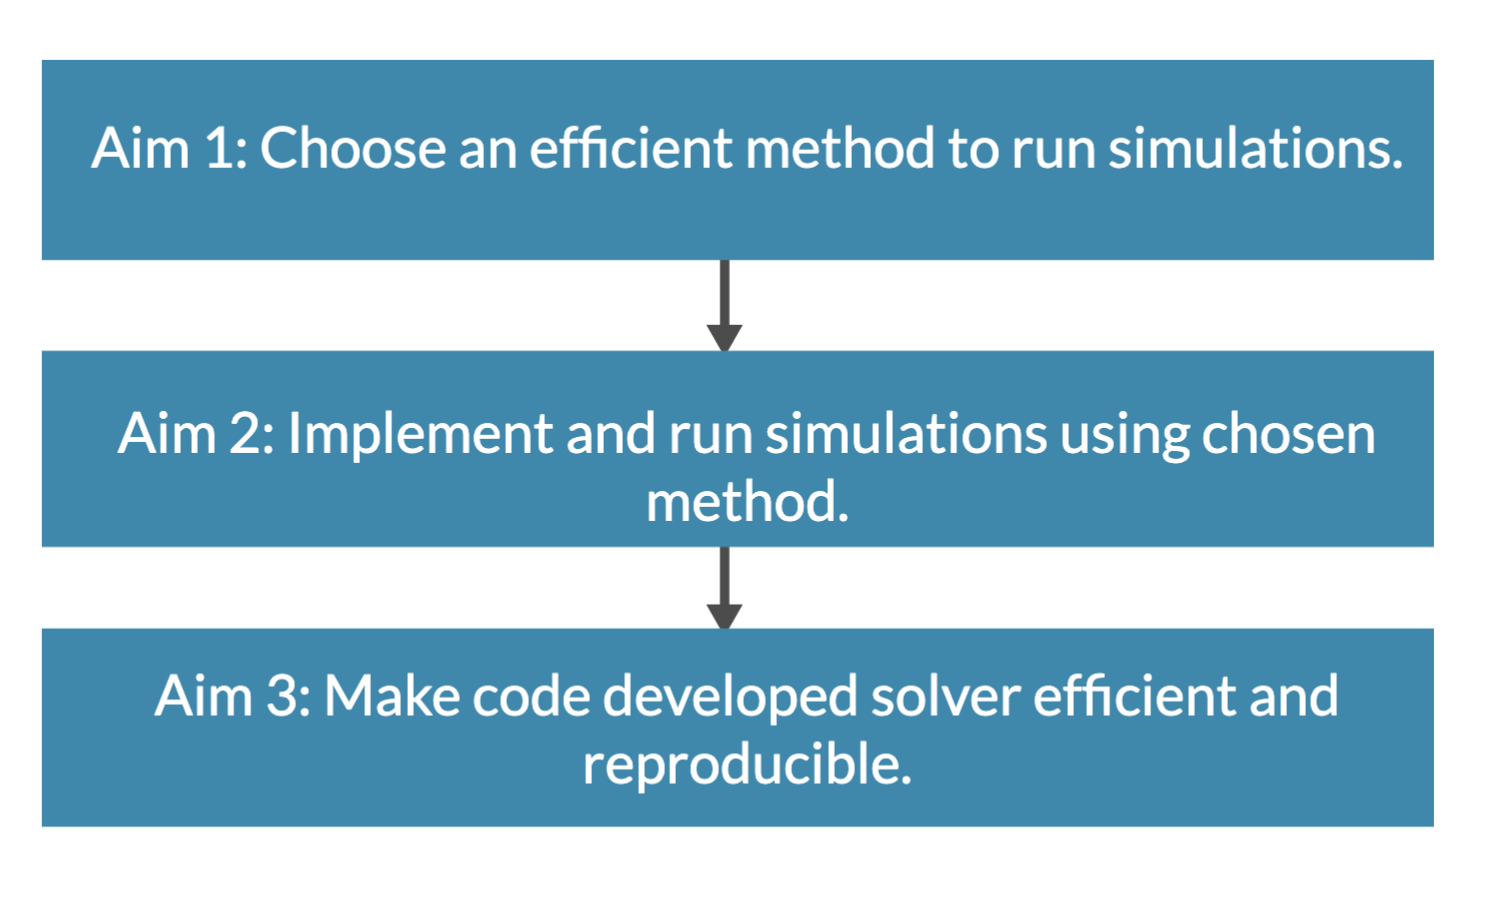
\includegraphics[width=12cm]{GWU_Thesis_Sarmakeeva/Images/chap1/Aims.png}
    \caption{Schematic overview of the study's aims.}
    \label{fig:aims}
\end{figure}
Three aims of this work and the methods that will be used to achieve them are provided below:

\textbf{Aim 1: Choose an efficient method to run simulations.}

In order to select the most appropriate and efficient method to run simulations, we need to consider several key aspects:
\begin{enumerate}
    \item \textbf{Coupling method:} Identify a suitable method for coupling the solid and fluid simulations, considering the characteristics of a landslide and granular media dynamic. This involved comparing different coupling techniques, such as one-way and two-way coupling, as well as investigating different levels of coupling, such as resolved and unresolved CFD-DEM approaches.
    \item \textbf{Free surface reconstruction:} It is necessary to evaluate various techniques for accurately capturing the free surface in multiphase flow simulations. This field is still quite tricky and needs careful consideration. To choose the most suitable method, it is necessary to compare different methods for free-surface reconstruction in terms of their accuracy, computational efficiency, and ease of implementation in the final solver.
    \item \textbf{Stability and robustness:} Assess the stability and robustness of the chosen methods, especially when considering the influence of the coupling between solid and fluid simulations. Stability and robustness may involve analyzing the convergence properties and sensitivity to numerical parameters such as time step and grid resolution.
    \item \textbf{Scalability and parallelism:} Investigate the scalability and parallel performance of the chosen methods, ensuring that they can effectively utilize available computational resources and accommodate large-scale simulations.
    \item \textbf{Implementation complexity:} Consider the complexity of implementing the chosen methods within an existing simulation framework or developing a new one. The challenges of implementing include assessing the compatibility of the methods with existing software libraries and tools, as well as the effort required for code development and maintenance.
\end{enumerate}

By carefully evaluating these factors, including the detailed assessment of various coupling methods in the context of fluid and granular media dynamics, advanced techniques for free surface reconstruction in multiphase flows, and the critical examination of stability, robustness, scalability, and implementation complexity, the most efficient method for running simulations should be chosen. This not only helps to achieve high-precision and reliable simulation results but also efficiently optimizes computational resources.

\textbf{Aim 2: Implement and run simulations using the chosen method.} 

The implementation phase should involve integrating third-party libraries or adapting existing ones to meet the specific requirements of our chosen simulation method. This phase is critical in ensuring that our simulations are not only theoretically sound but also practically feasible. Following the implementation, it is imperative to establish a robust verification and validation (\ac{V&V}) process. This process would involve rigorous testing against known benchmarks to ensure the simulations accurately represent the physical phenomena of interest. Including a parallel computing option is crucial for optimizing performance, particularly given the computationally intensive nature of landslide simulations.

Once the implementation is validated, we will proceed with a detailed analysis of the simulation results. This includes evaluating the solver's physical accuracy, computational efficiency, and overall stability. A grid convergence study will be integral to this analysis, providing vital insights into the solver's numerical stability and accuracy.
The final step involves applying our simulation framework to real-world scenarios, akin to the experiments detailed in \cite{mao2020resolved} and \cite{shen2022resolved}, where a granular mass interacts with a fluid. 

This will test the effectiveness and applicability of our simulations in real-world conditions and contribute valuable insights into the dynamics of granular materials in fluid environments, thereby bridging the gap between theoretical modeling and practical application.

\textbf{Aim 3: Make code developed solver efficient and reproducible.}

The final aim was to create a repro-pack following a tradition of reproducible research at Barba's group \cite{barba2018terminologies}, \cite{Mesnard2023}. The source code, which is used for simulations and post-processing scrips, should be easily accessible on GitHub \cite{github} along with container image \cite{Docker_introduction} to reproduce the main experiments. The container image encapsulates all dependencies, allowing others to replicate the main experiments. A container image is essentially a lightweight, standalone, and executable package that includes everything needed to run a piece of software, including the code, a runtime environment, libraries, environment variables, and configuration files. Containers are isolated from each other and from the host system, ensuring that they are consistent across different environments and reducing conflicts between different software running on the same system.

Any initial conditions, boundary conditions, and material properties necessary for the simulations are documented, as well as detailed instructions on how to run the simulations, including necessary command line arguments or configuration settings provided in an image. Detailed explanations of the theoretically used model are provided in the next chapter, and the implementation of the code and the interpretation of results are provided in Chapter 3. The implementation is done by developing force with third-party libraries or modifying existing ones. After implementation, the model is supported by a verification and validation procedure. The grid convergence study also supports the stability of the solver. After that, the solver tested running multi-spherical bodies interacting with fluid, and the last step was an application to real-world problems to test its effectiveness and usefulness. It was an experiment where a granular mass fell into the water as in works \cite{mao2020resolved} or \cite{shen2022resolved}.

\section{Literature review}

The field of landslide research is vast, but only a few academic papers and computational approaches have been proposed in recent years. The primary criterion for the simulation aspect of this study was to build a stable solver and to ensure that open-source code was used to support the requirement for reproducibility. As the landslide process involves a solid component interacting with fluid, it was necessary to choose the most suitable method for simulating solid and fluid components with a free surface in an optimized and compatible manner. It is essential to consider the variety of free surface reconstruction methods available, as they differ in terms of numerical stability and the ability to capture the interface between fluids as well as being stable to be able to couple with solid part. 

\begin{figure}[!ht]
    \centering
    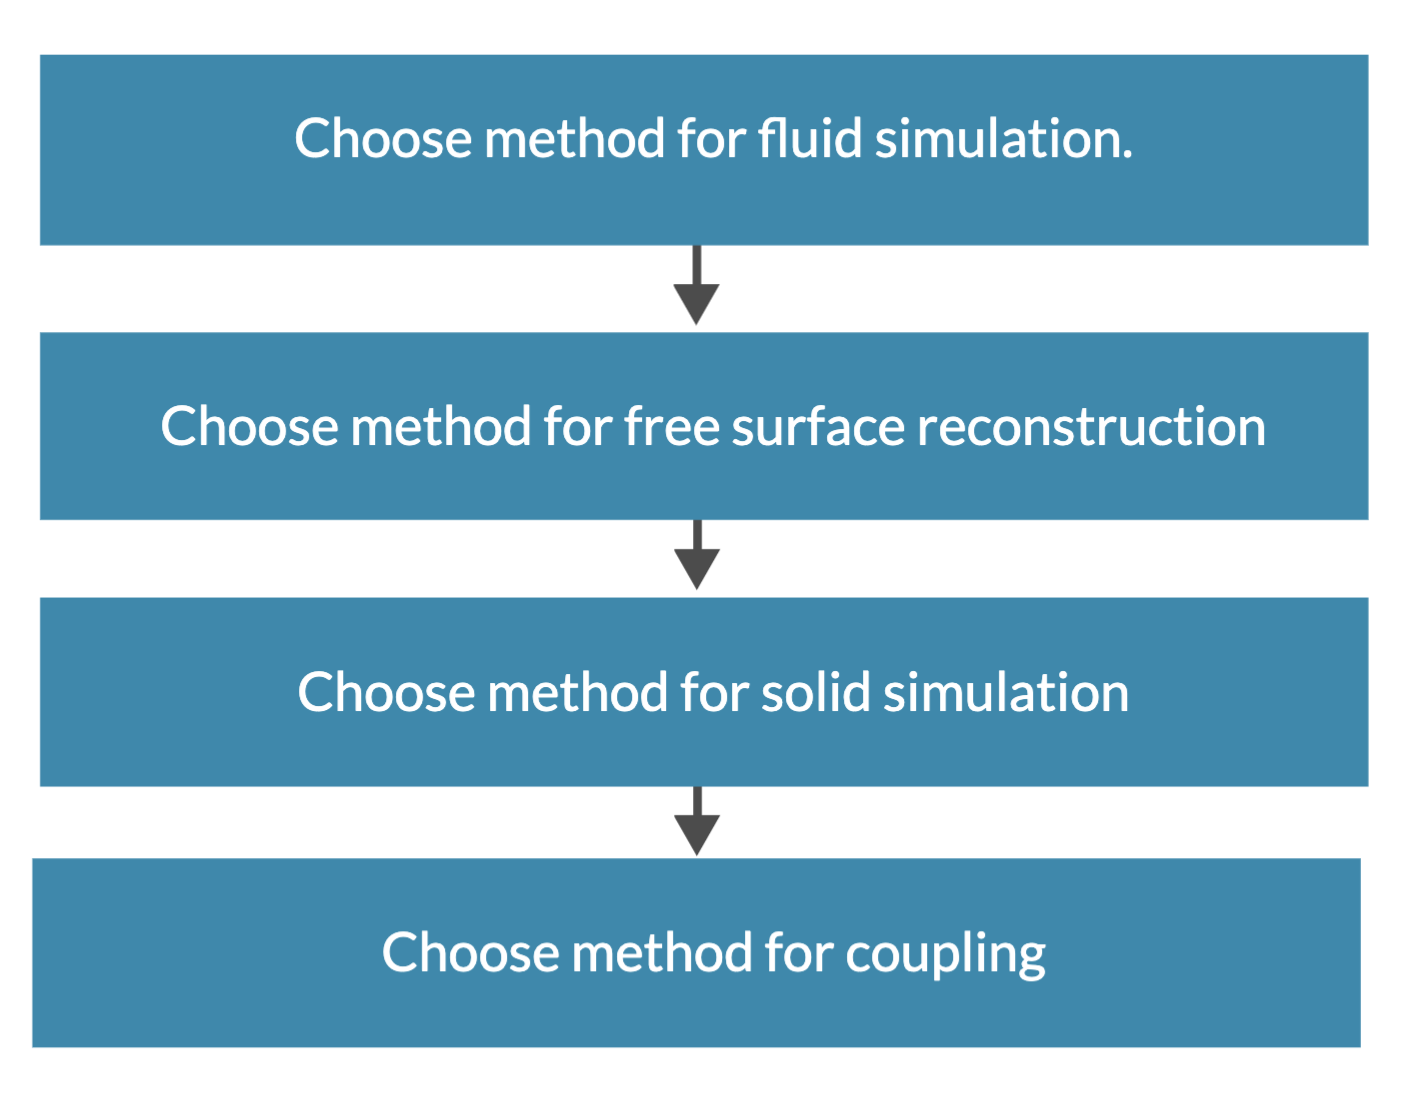
\includegraphics[width=10cm]{GWU_Thesis_Sarmakeeva/Images/chap1/lit_rew.png}
    \caption{Schematic description of methods which is necessary to review.}
    \label{fig:aims}
\end{figure}

The process of finding the most suitable approach to solve our problem consisted of deciding the best method for simulation; it turned out that only coupling solid and fluid parts was a suitable solution. This led to a question of which method could be used for fluid simulation, which in turn raised a question about the method for free surface simulation and its difficulties due to instabilities caused by surface tension. Last but not least, deciding how we would simulate solid and arbitrarily shaped bodies was necessary.

\section{Methods for fluid simulation}

Fluid simulation is a crucial area of research in many industries, from engineering to meteorology. Fluid simulation methods play a vital role in designing more efficient aircraft, predicting weather patterns, and many other applications. Researchers use various methods for fluid simulation, including Smoothed Particle Hydrodynamics (\ac{SPH}) \cite{gingold1977SPH, monaghan1994SPH}, Finite Element Method (\ac{FEM}) \cite{lewis2004fundamentals}, Volume of Fluid (\ac{VOF}) \cite{hirt1981volume}, and Lattice Boltzmann Method (\ac{LBM}) \cite{chen1998lattice}. Schematic description of existing methods shown in Figure \ref{fig:methods_for_fluids}.
\begin{figure}[!ht]
    \centering
    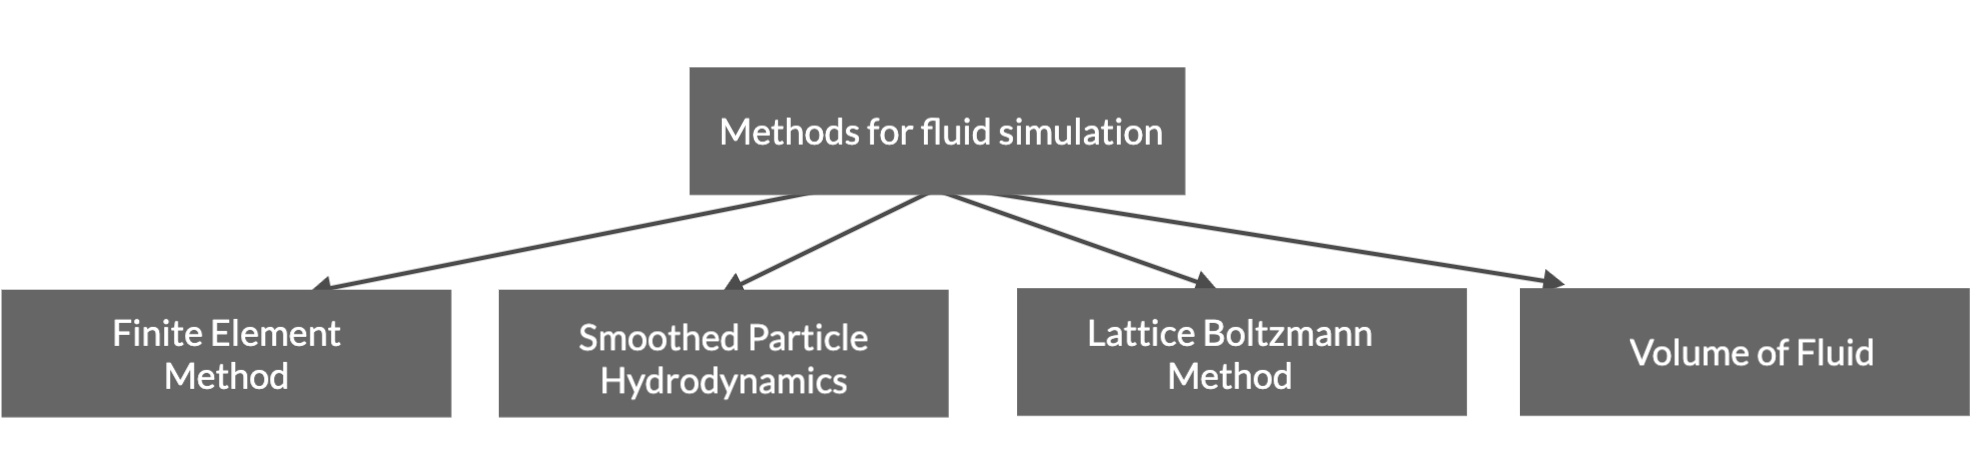
\includegraphics[width=15cm]{GWU_Thesis_Sarmakeeva/Images/chap1/methods_for_fluids.png}
    \caption{Schematic description of methods for multiphase flow simulation.}
    \label{fig:methods_for_fluids}
\end{figure}
Each method has its advantages and limitations, and researchers choose the appropriate method based on the specific needs of their research. SPH is a mesh-free, Lagrangian method useful for simulating free-surface and multiphase flows. The LBM is also a meshless approach, and it is a relatively new method that is gaining popularity due to its ability to simulate complex fluid flow phenomena. FEM is a widely used method for solving fluid mechanics problems in complex geometries. The VOF is a method that tracks the interface between fluids and is useful for simulating free-surface flows.

\subsection{Smoothed Particle Hydrodynamics}

Smoothed Particle Hydrodynamics (SPH) is a Lagrangian method that models fluid as a collection of particles that interact with each other based on their relative positions and velocities rather than mesh cells. The central concept is that fluids are simulated by discrete particles, and their movement is prescribed by the flow field. SPH has proven effective in simulating fluid flows with complex geometries and free surfaces \cite{adami2012SPH}, such as ocean waves \cite{barreiro2013SPH} and splashing water \cite{moreira2020SPH}. For the current research, we consider incompressible fluid; there are two general approaches in the literature with small compressibility - Weakly Compressible SPH (WCSPH)\cite{ren2015nonlinear} and flow simulated by enforcing the incompressibility -  Incompressible SPH (ISPH) \cite{macia2012boundary}. 

To simulate two-way coupling, we considered pressure on a solid body; however, in SPH, it leads to a couple of problems. Special boundary conditions are needed to set solid body boundaries, which is a well-known and non-trivial issue. In the work \cite{kopysov2015modeling}, it was found that WCSPH is more stable and accurate than ISPH for the pressure calculation on solid boundaries. We used dualSPHysics code \cite{Dual_SPH2019accuracy} the work \cite{kopysov2015modeling} to run an evaluation of the method.

\begin{figure}[!ht]
    \centering
    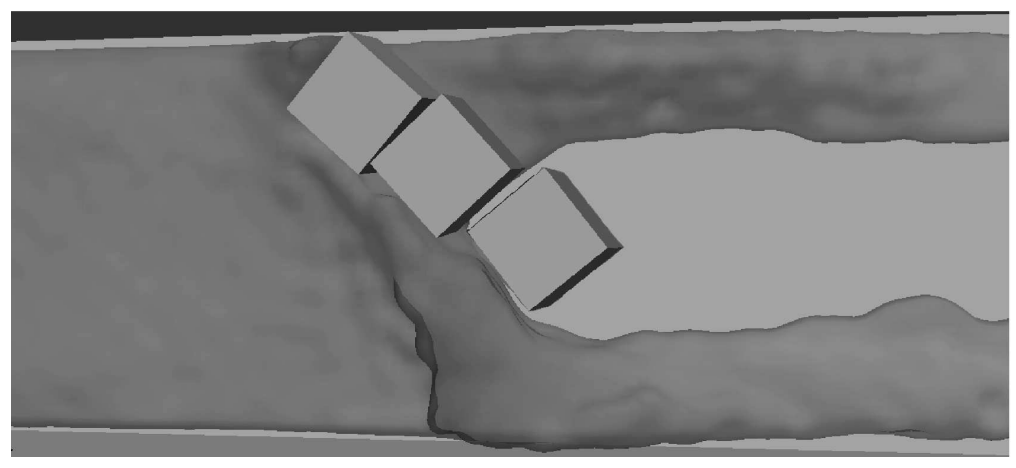
\includegraphics[width=16cm]{GWU_Thesis_Sarmakeeva/Images/chap1/3_blocks_SPH.png}
    \caption{Simulation with \cite{Dual_SPH2019accuracy} from the \cite{sarmakeeva2017meshfree}.}
    \label{fig:3_blocks_SPH}
\end{figure}

The method requires a large number of particles to accurately capture the free-surface dynamic, which can result in high computational costs and make it challenging to simulate larger-scale systems. Another area for improvement of SPH is that it relies on artificial viscosity to handle fluid viscosity, which can lead to inaccurate results, especially when the flow is complex \cite{zhang2018dualsphysics}. 

The artificial viscosity can also cause unwanted damping effects on the fluid motion. Furthermore, SPH struggles with accurately modeling fluid-solid interactions \cite{Dual_SPH2019accuracy}, causing inaccuracy in boundary treatment. The placement of boundary particles, for instance, can affect the accuracy of the results, and it can be challenging to represent complex geometries correctly. As shown in Figure \ref{fig:3_blocks_SPH}, from the work \cite{sarmakeeva2017meshfree}, where provided results of a simulation for three falling blocks and fluid with SPH method conducted with the open-source code DualSPHysics \cite{Dual_SPH2019accuracy}. The work provided analysis for multiple solid bodies interaction, where blocks moved with fluid. Results compared with physical experiments and for the block center mass results are in good agreement. However, the fluid simulation results indicate that boundary conditions can be a concern since the fluid does not flow through gaps between solid bodies. For this reason, we considered other methods for fluid simulation.

\subsection{Finite Element Method}
The Finite Element Method (FEM) is an Eulerian method that discretizes the fluid domain into finite elements \cite{FEM}, where a set of equations represents fluid properties. This method is particularly effective for simulating complex fluid flows, which is part of the problem in a seashore area. FEM can handle complex geometries and boundary conditions and has been widely used in simulating fluid-structure interactions.

The first step in FEM is to discretize the domain of the fluid flow problem. This involves dividing the fluid region into a mesh of small, interconnected elements, typically triangles in 2D and tetrahedra or hexahedra in 3D. Each element is assumed to represent the fluid properties within its boundaries. Fluid dynamics is governed by the Navier-Stokes equations, which describe the motion of viscous fluid. In FEM, these equations are applied to each element of the mesh. Within each element, interpolation functions (shape functions) are used to approximate the fluid properties (such as velocity, pressure, and temperature) across the element. These functions are defined so that they are simple within an element and match up with the neighboring elements to ensure continuity. 

The Navier-Stokes equations are transformed into an integral form using the Galerkin method. This involves multiplying the governing equations by a test function (which is often the same as the shape function) and integrating over each element. This process converts the differential equations into a set of algebraic equations. The equations for each element are assembled into a global system of equations that represent the entire fluid domain. This system is then solved using numerical methods, such as the Newton-Raphson method or other linear/nonlinear solvers, to find the approximate solution to the fluid flow problem. The resulting solution provides values of fluid properties at discrete points in the mesh. Post-processing techniques are used to interpret these results, allowing for visualization and analysis of the flow field, pressure distribution, and other relevant physical quantities.

The advantage of FEM is that this method is highly versatile and can handle complex geometries and boundary conditions. The method provides good accuracy and convergence properties, is well-suited for non-uniform meshes, and can adaptively refine the mesh in regions requiring higher resolution. The incorporation of solid bodies into finite element mesh could be beneficial.

However, FEM requires a high level of mesh refinement to accurately capture the fluid behavior near solid boundaries, which can result in significant computational overheads \cite{FEM_2} especially for granular media. FEM also can be computationally intensive, primarily for 3D problems and fine meshes, and the quality of the solution is highly dependent on the quality of the mesh. Due to this reason, we did not consider this method for our work.

\subsection{Lattice Boltzmann Method}
 
The Lattice Boltzmann Method (LBM)\cite{begum2008lattice} is a relatively new method to simulate the interaction between different fluid phases, such as liquid and gas. LBM has demonstrated excellent performance in simulating fluid flows with complex geometries and boundary conditions and is particularly useful in modeling microfluidic systems \cite{aidun2010lattice}. The method is based on the concept of simulating fluid flow by tracking the evolution of particle distribution functions on a lattice grid. Each particle carries a fraction of the fluid's mass and momentum, and the macroscopic flow properties are derived from these microscopic particle interactions.

The simulation domain is discretized into a lattice grid. Each node on the lattice represents a set of discrete particle velocities. In LBM, these velocities are chosen so that particles can only move to adjacent lattice nodes during each time step. The method involves two main steps: collision and streaming. During the collision step, particles at each lattice node interact, redistributing their velocities according to specific rules (collision operators). In the streaming step, particles move to adjacent nodes based on their new velocities.

To simulate multiphase flows, LBM incorporates additional forces or rules to account for the interactions between different phases. Common approaches include the Color-Gradient Model \cite{ba2013color}, where different colors are assigned to other fluids, and a color gradient is used to model surface tension. Shan-Chen Model \cite{huang2011forcing} introduces an interaction potential between particles to mimic the cohesive and adhesive forces in multiphase flows. Phase-Field Model \cite{takada2013phase}uses a continuous phase-field variable to represent different phases and simulate the interface dynamics.

Surface Tension and Wetting Important aspects of multiphase flows are modeled by incorporating additional terms in the LBM equations that represent intermolecular forces. The interface between different fluid phases is tracked and evolved over time, which is critical in accurately capturing the physics of multiphase flow, such as droplet formation, breaking, and coalescence.

LBM is particularly advantageous for multiphase flows due to its ability to easily incorporate complex boundary conditions, handle interfacial dynamics, and adapt to parallel computing frameworks, making it suitable for large-scale, high-resolution simulations.

One of the challenges in LBM for multiphase flow is ensuring numerical stability, especially for high density and viscosity ratios between the phases. Moreover, accurately capturing the microscale interactions at the interface can be computationally demanding, and simulating arbitrarily shaped bodies using LBM could be quite complicated.

\subsection{Finite Volume Method}

Finally, the Finite Volume Method (\ac{FVM}) is a well-established numerical method for simulating fluid flows. In FVM, the computational domain is divided into small, discrete control volumes. These volumes are typically shaped as simple polygons (or polyhedra in 3D), covering the entire domain without overlapping. The governing equations for fluid flow, primarily the Navier-Stokes equations, are converted into their integral forms. This allows the equations to be applied over each control volume, ensuring the conservation of mass and momentum within each volume.

Flow properties such as velocity, pressure, and phase fractions are volume-averaged within each control volume. These average values are used to represent the state of the fluid within the volume. Multiphase flows are complex due to the interactions between different phases. FVM handles this by incorporating models that capture these interactions with methods like the Volume of Fluid (VOF) to track the interface between phases. 

The VOF is an Eulerian method that tracks the fluid interface by solving a transport equation for each fluid phase with different density parameters. The method marks cells with values between $0$ and $1$. In the VOF, surface tension effects are modeled by introducing a surface tension force into the momentum equations. This force is typically applied at the fluid interface, where a significant role plays the volume fraction gradient. Accurate calculation of the interface curvature is essential for correctly modeling the surface tension force. The curvature is generally computed from the gradients of the volume fraction field. Numerically, this can be challenging, especially in complex flow situations with highly deformed interfaces.

Various improvements of VOF have been suggested to handle complex geometries, free surfaces, and multiphase flows, such as the Marker and Cell method \cite{mac}, Geometric Reconstruction \cite{VOF_reocnstr}, High-Resolution Interface Capturing \cite{HIRC}, or Level Set \cite{VOF_level_set}. This method is discussed more thoroughly in the following sections. 

However, capturing the dynamics of the phase interface, especially in scenarios with complex topological changes like breaking waves or droplet coalescence, can be challenging. Another problem with the method is that high computational costs for satisfactory mesh resolutions are necessary for capturing small-scale interfacial phenomena. 

The FVM naturally conserves mass and energy, which is crucial for accurate multiphase flow simulations. It can handle complex geometries and is adaptable to structured and unstructured meshes, which is essential when large solid masses interact with multiphase fluid.

After analyzing the strengths and weaknesses of SPH, LBM, FEM, and FVM, we have determined that the VOF method aligns most closely with the requirements for our simulation. The VOF method's robustness in handling multiphase flows and its ability to track the interface between multiple phases accurately make it particularly suitable. However, a crucial aspect of our upcoming work involves selecting the most effective technique for free-surface reconstruction. This step is essential for ensuring the precision and reliability of simulation, especially in scenarios where surface tension and interfacial dynamics play significant roles. Our choice will be guided by a balance between computational efficiency, numerical stability, and the ability to handle the incorporation of the third phase - solid bodies.

\section{Method for free-surface representation} %free surface simulation

The free-surface simulation took a significant time for the research. Several methods are available for simulating free-surface flows, each with advantages and limitations. There are two general approaches when using the Finite Volume Formulation (or considering Eulerian formulation): interface-tracking methods and interface-capturing. Figure \ref{fig:vof_methods} provided the general situation with existing methods for free surface simulation for multiphase flow simulation. We highlighted the Front Tracking Method (FTM)\cite{front-tracking} and the Marker and Cell (MAC) Method \cite{mac} as the main approaches for interface tracking. For interface tracking methods, the field is waste. Because there are so many methods for free surface reconstruction, we had a special interest in mindfully choosing the most suitable approach.

\begin{figure}[!ht]
    \centering
    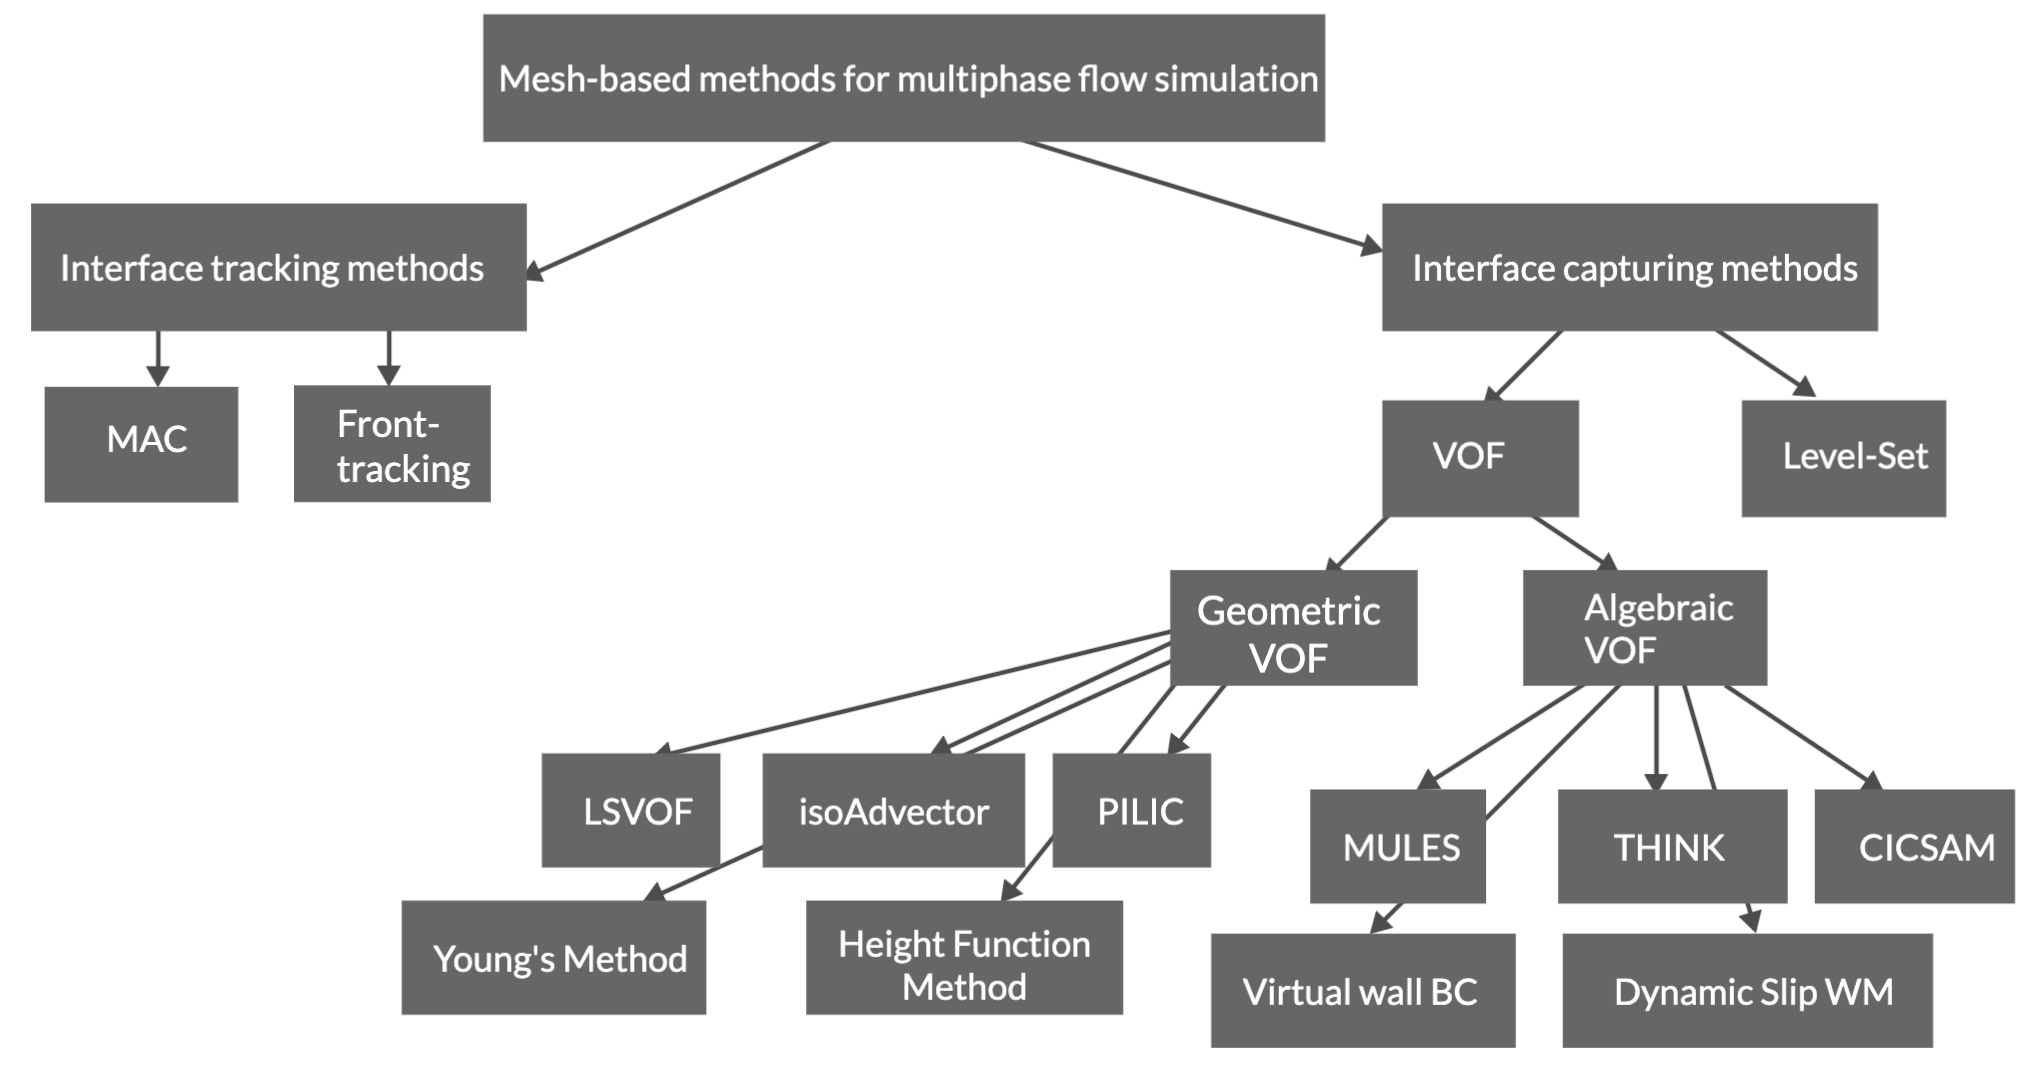
\includegraphics[width=16cm]{GWU_Thesis_Sarmakeeva/Images/chap1/VOF_methods.png}
    \caption{Schematic description of existing in the literature for Volume of Fluid methods.}
    \label{fig:vof_methods}
\end{figure}


\subsection{Interface Tracking Methods}

The first category includes the Front Tracking Method (\ac{FTM})\cite{front-tracking} and Marker and Cell (\ac{MAC}) Method \cite{mac}. While interface-tracking methods could be effective in some scenarios, they have fundamental disadvantages compared to interface-capturing methods. One of the most important ones is the limited ability to handle topological changes such as merging, breaking, or creating new interfaces, which can be challenging. Such events often require advanced mesh manipulation techniques, which can be difficult to implement and may introduce instabilities. This aspect is important when solid granular material will be falling into the water.

Although \ac{CFD} is generally complex, interface tracking methods often involve complex algorithms and data structures to track and manage the moving interface mesh or markers explicitly. This can lead to high computational costs and require a large amount of memory and processing time.
Ensuring good mesh quality and resolution near the interface is critical for interface tracking methods. Maintaining an optimal mesh can be difficult, especially in large deformations or high curvature cases. Due to the complexity of managing the interface mesh or markers, interface tracking methods can be more challenging to parallelize and scale efficiently on high-performance computing systems.

\subsection{Interface Capturing Methods}

In contrast, the interface-capturing methods are like algebraic \cite{algebraicVOF}, geometric VOF \cite{roenby2019isoadvector} formulation and Level Set Method (\ac{LSM}) \cite{VOF_level_set}. A group of sharp interface methods \cite{sharp-interface} offers a more straightforward and flexible approach to handling complex topologies with potentially lower computational costs than level-set methods. However, they may suffer from a smeared interface representation and require additional techniques to sharpen the interface and maintain mass conservation.

Some well-known geometric reconstruction methods include the Piece-wise Linear Interface Calculation (\ac{PLIC}) \cite{huang2012piecewise} method, which reconstructs the interface as a line in 2D or a plane in 3D within each interfacial cell. The PLIC is one of the most widely used methods for reconstructing interfaces in VOF simulations. The Height Function Method \cite{height-function} reconstructs the interface by calculating the height of the fluid in each cell, which is then used to derive the interface normal and curvature. This technique is particularly effective in structured Cartesian meshes. Youngs' Method \cite{youngs-method} represents the interface as a piece-wise linear surface within each cell, allowing for time-dependent multi-material flow simulations with significant fluid distortions. The isoAdvector \cite{roenby2019isoadvector} method involves two main steps: exploiting an iso-surface concept for modeling the interface inside cells in a geometric surface reconstruction step and modeling the motion of the face-interface intersection line for a general polygonal face to obtain the time evolution within a time step of the submerged face area. As a plus, it has an open-source implementation as a part of OpenFOAM \cite{jasak2007openfoam}.

These are just a few examples of the geometric reconstruction schemes used in multiphase flow simulations. Each method has its advantages and disadvantages, and choosing the most suitable method depends on factors like the problem's complexity, computational resources, and accuracy requirements.

Algebraic reconstruction schemes are used in interface capturing methods, particularly within the context of the Volume of Fluid (VOF) method. These methods compute the fluxes algebraically without the need for geometric reconstruction of the interface. Some well-known algebraic reconstruction methods include compressive schemes, which use the information of the interface's orientation (interface normal) with respect to the cell face to compute the face flux. 

One example of a compressive scheme is the High-Resolution Interface Capturing (\ac{HIRC}) method \cite{HIRC}. Tangent of Hyperbola for Interface Capturing (\ac{THINC}) \cite{THINC} schemes utilize a hyperbolic tangent function to represent the phase indicator function. The volume fraction is then obtained using a numerical approximation, such as volume-averaged, polynomial, or hyperbolic tangent representation. The \ac{CICSAM} (Compressive Interface Capturing Scheme for Arbitrary Meshes)\cite{CICSAM} is an extension of the compressive VOF method for unstructured meshes. It uses the orientation of the interface normal to compute the face flux. Slope-Limiter-Based Methods \cite{liu2021new} use slope limiters to control the steepness of the volume fraction gradient within the cells, which helps to avoid numerical oscillations and maintain the sharpness of the interface. Multidimensional Universal Limiter for Explicit Solution (\ac{MULES})\cite{MULES} is a numerical scheme where the advection term is modified to compress the surface and reduce smearing. It helps achieve a higher-order scheme for a more accurate advection at the surface. These algebraic reconstruction schemes offer varying degrees of accuracy and computational efficiency. The choice of the most suitable method depends on factors like problem complexity, computational resources, and accuracy requirements. 

Although based on our experience of using this approach in OpenFOAM \cite{MULES}, the method does not fully capture the movement of the free surface and the formation of droplets, and the method provided in \cite{roenby2019isoadvector} shows better simulation results.

The Level Set method is a popular numerical technique used for tracking interfaces and shapes in various applications, including two-phase flow simulations. It applies widely to multiple problems, including fluid mechanics, computer graphics, and image processing. The method has its advantages, such as accurate computation of interface properties. The technique allows precise calculation of normals and curvature, which are crucial in many interfacial flow applications. Another benefit of the method is implicit interface representation, which makes it easier to handle complex topologies such as merging, breaking, and self-intersecting interfaces. The Level Set method can be easily extended to work with Adaptive Mesh Refinement (AMR), allowing for better resolution in areas of interest and reduced computational cost.

On the other hand, several disadvantages may make the method not the first choice. One of the most significant issues is that it does not inherently conserve mass for each phase, a critical requirement in the numerical modeling of realistic two-phase flows. Although there are techniques to limit mass loss, the problem cannot be eliminated entirely. Moreover, solving the Level Set equation can be computationally expensive, especially for large-scale problems or those requiring high accuracy, and the Level Set function needs to be reinitialized frequently to maintain a signed distance function, which can introduce additional computational overhead and may lead to a loss of accuracy. Coupling the Level Set method with other physics, such as fluid flow, can be challenging and may require additional numerical techniques to address issues like mass conservation or surface tension.

Based on the literature review, the most general and accurate method is the geometric VOF; it has implementation as an OpenFOAM solver \cite{roenby2019isoadvector}, which is called IsoAdvector. The method was chosen for free surface reconstruction and compared with available in OpenFOAM MULES \cite{MULES}. Because of the complexity of the technique, it is necessary to describe it in more detail, which will be done in the next chapter.

The isoAdvector method is unique for a couple of reasons: First, it uses a special way to draw the boundary line inside a cell when we are looking at how a liquid's surface changes. Secondly, it tracks how this outlined surface moves across the cell's boundary over time. By figuring out how much of the boundary gets wet during a certain period, we can precisely calculate the amount of liquid that's moved through it.

Due to open source availability and good performance of the method during the testing phase and the that we considered finding the boundary of solid bodies and existing gaps between solid bodies, which are consequences of the boundary condition problem in the SPH method, we concluded that isoAdvector would be the best choice for our simulation.

\section{Methods for granular media simulation}

Several methods are available for simulating granular media, each with advantages and limitations. These methods include the Discrete Element Method (DEM)\cite{cundall1979discrete}, Finite Element Method (FEM), Smoothed Particle Hydrodynamics (SPH)\cite{monaghan1994SPH}, Lattice Boltzmann Method (LBM) \cite{chen1998lattice} \cite{begum2008lattice}, and Molecular Dynamics (\ac{MD}).

\subsection{Discrete Element Method}
The DEM is a method widely used for studying the behavior of granular materials under different loading conditions. In this approach, granular media are modeled as a collection of discrete particles interacting with each other through contact forces. One of the strengths of DEM is its ability to capture the details of individual particle interactions and calculation of contact forces, making it suitable for studying granular materials with complex geometries and boundary conditions.

In DEM, granular materials are modeled as an assembly of discrete particles. Each particle is treated as a distinct entity with its own properties (such as mass, size, and shape). The core of DEM is the calculation of forces and torques when particles come into contact. The method uses contact mechanics models to simulate the interaction forces, including normal force (due to collision), tangential force (due to friction), and possibly other forces like cohesion. Newton's laws of motion govern the motion of each particle. The forces and torques resulting from particle interactions determine the acceleration, which is then used to update the velocity and position of each particle over time. DEM employs a time-stepping algorithm to solve the motion equations iteratively. At each time step, the method updates the position and velocity of each particle based on the net forces acting on it. 

DEM excels in capturing the details of particle-particle and particle-wall interactions, and the method can effectively model granular materials flowing through or interacting with complex geometries. It's also suitable for various materials with different properties, including cohesion, friction, and irregular shapes. Parameters such as particle size distribution, shape, and material properties can be tailored to simulate a specific type of granular material accurately.

However, DEM is computationally demanding, especially as the number of particles increases. This is due to the need to calculate interactions for each particle pair at every time step. While DEM is excellent for granular materials, it may only accurately capture the behavior of materials with significant cohesive or adhesive forces with additional modeling considerations. DEM could be useful for its ability to detail individual particle interactions, which is essential for understanding the behavior of granular materials. Its ability to model complex particle geometries and interactions makes it a powerful method. 

In contrast, FEM is useful for simulating large-scale systems with solid bodies, complex geometries, and boundary conditions. While FEM can capture the behavior of granular materials under different loading conditions, it is less accurate in capturing the details of individual particle interactions.

The Smoothed Particle Hydrodynamics Method could be used not only for fluid simulation but also for predicting the behavior of granular media as a fluid with individual particles representing the grains. This method is well-suited for simulating the dynamics of granular flows and mixing processes. However, its accuracy in capturing the detailed contact forces between individual particles is limited, which restricts its applicability to certain granular materials.

Lattice Boltzmann Method falls into the same category as the SPH group of methods. It is an efficient method for simulating large-scale systems with complex geometries and can accurately capture the fluid-like behavior of granular materials. However, it can be computationally expensive for high-resolution simulations, and its accuracy in capturing the detailed contact forces between individual particles is limited.

Molecular Dynamic Methods help study the behavior of granular materials at a microscopic scale and can capture the effects of thermal fluctuations and chemical reactions. However, it is computationally expensive and may need to be more practical for simulating large-scale granular systems.

Considering each method's strengths and limitations, we have chosen DEM featuring multi-spherical bodies, called clumps in the literature, as our method for simulating granular media. DEM can capture the details of individual particle interactions and contact forces, and adding clump features allows for the modeling of cohesive forces between particles, which can be crucial in certain types of granular materials. 

\section{Coupling approach.}

Coupling methods are commonly used in simulations where multiple physical phenomena are involved. There are different ways to couple simulations; each method has advantages and disadvantages. Some common coupling methods include one-way coupling, two-way coupling, and fully coupled simulations.

In one-way coupling, one simulation provides input to another, but the second simulation does not affect the first. This method is useful when one simulation has a negligible effect on the other simulation. In two-way coupling, which sometimes is called strong coupling, both simulations interact with each other, and the results of each simulation affect the other. However, the interactions between the simulations are limited to specific points in time, and the simulations do not interact with each other at every time step. In fully coupled simulations, the models are completely integrated, and the results of both simulations are obtained simultaneously. The simulations interact at every time step, and each simulation considers the other simulation's effect.

\subsection{Immersed Boundary Method}.
There are not a lot of options on how to implement coupling for this type of problem. Because we can not incorporate solid body mesh into the fluid mesh or generate body conformal mesh, every time step would be very cumbersome on top of the already existing computational load. 

The most well-known approach for two-way coupling is the Immersed Boundary Method (\ac{IB}) \cite{mittal2005immersed}. One of the key strengths of the IB method is its ability to simplify the computational modeling of complex, moving, or deforming boundaries. This is achieved by embedding the structure (boundary) within a regular fluid grid, eliminating the need for the fluid mesh to conform to the shape of the solid boundary. It applies to a wide range of problems, from biological applications like blood flow through arteries and heart valve dynamics to engineering applications like fluid interaction with flexible structures or porous media. The IB method typically uses a mathematical formulation to couple the fluid and solid equations, where forces are incorporated into governing equations and are exchanged between the fluid and the immersed boundary. This results in a seamless integration of solid and fluid dynamics, allowing for the accurate capture of their interaction. 

While the IB method offers distinct advantages, it also faces challenges, particularly in accurately capturing the boundary layer dynamics and ensuring numerical stability for highly stiff structures. These challenges require special numerical treatment and sometimes integration with other computational techniques. 

There are a couple of approaches to projecting the force onto fluid mesh - the Continuous Forcing Approach and the Discrete Forcing Approach. The first is how IB initially came into use - for elastic boundary simulation. Utilizing the Continuous Forcing Approach in scenarios involving flows with rigid bodies presents specific difficulties, primarily because the behavior of the forcing terms can become problematic in rigid scenarios. To address this issue, simplified models are designed to approximate the influence of the solid boundary on the fluid flow. Nonetheless, these models introduce specific parameters that can significantly impact the simulations' numerical accuracy and stability. An inherent characteristic of these methods is the smoothing of the forcing function, which may lead to a less distinct representation of the Immersed Boundary (IB). This lack of sharpness can be particularly challenging in simulations involving high Reynolds number flows. Furthermore, a common requirement of these methods is solving the governing fluid dynamics equations within the immersed body, adding another layer of complexity to the simulation process. 

In turn, the Discrete Forcing Approach is where solid body boundaries are applied to computational cells. There are two ways of imposing boundary conditions - indirect and direct. In the first case, the process involves modifying the numerical solution by subtracting forcing functions after the discretization of the Navier-Stokes equations. A key benefit of this method is the elimination of the necessity to pre-define parameters for the forcing functions before solving the Navier-Stokes equations. Additionally, it avoids stability issues often associated with continuous forcing functions. However, this approach still requires the implementation of distributed forcing functions, which rely heavily on the chosen discretization algorithm. This reliance underscores the method's dependency on the specifics of the numerical discretization process.

It is a way more popular direct imposition of boundary conditions. In this approach, the boundary is defined by a set of Lagrangian points. The fluid velocities at these points are interpolated and utilized to determine their movement. Subsequently, a constitutive equation calculates a force term, which is then distributed to the adjacent cells. This method effectively integrates the movement of the boundary with the fluid dynamics, ensuring a cohesive interaction between the fluid and the boundary defined by the Lagrangian points. 

One of the ways of direct imposition of boundary conditions is a ghost-cell method, where fictitious cells are located inside the solid body in a computational mesh. These ghost cells are used to impose boundary conditions at the fluid-structure interface. The approach extends the computational domain into the solid body, allowing for a more straightforward application of boundary conditions. The boundary of the immersed object is handled by modifying the fluid variables in these ghost cells to enforce the no-slip condition at the fluid-structure interface. This modification effectively creates a boundary layer that mimics the physical presence of the solid structure within the fluid flow. 

One of the main advantages of this method is its ability to provide a sharp representation of the boundary, which is particularly important for accurately capturing the flow characteristics near the boundary. It also helps maintain a more structured grid, which can be advantageous for numerical stability and simplicity in implementing the solver. While effective, the method can be computationally intensive, especially for complex geometries or highly dynamic interactions. Ensuring the accuracy of the ghost cell data and maintaining numerical stability are also important considerations in the implementation of this method.

In the cut-cell IB, in this method, The boundaries of the immersed body intersect cells on the CFD mesh. These intersected cells are known as "cut cells." The boundary of the structure effectively "cuts" through these cells, dividing them into fluid and solid portions. Once the cut cells are identified, they are modified to account for the part of the cell volume that is occupied by the solid structure. This involves adjusting the volume fractions of these cells to reflect the fluid and solid portions. The fluid equations are then solved only in the fluid portion of these cut cells. Boundary conditions are directly applied at the interface within the cut cells, depending on the nature of the fluid-structure interaction.

The fluid flow is simulated across the entire grid, including regular and cut cells. The presence of the structure is accounted for in the cut cells, allowing the fluid to interact realistically with the boundaries of the structure. One challenge of the Cut-Cell method is the potential creation of very small cut-cell fractions, which can lead to numerical instability. Various techniques, such as cell merging, flux correction, or stabilization algorithms, are employed to overcome these challenges. 

The advantage of this method is its ability to provide a high degree of accuracy in representing the geometry of the immersed structure. This is crucial in applications where the precise shape and position of the structure significantly affect the fluid flow. The Cut-Cell method is particularly beneficial in scenarios where the structure's geometry is complex or where the boundaries are not aligned with the main flow direction. It enables detailed and accurate simulations without complex meshing around the structure. 

For coupling with rigid bodies, the discrete forcing approach is more popular and suitable. Two ways of imposing boundary conditions on the immersed boundary are indirect and direct.

In our work, we have chosen to use two-way coupling. In this way, the method would allow us to simulate the interactions between different physical phenomena while being computationally efficient. This choice will provide the necessary level of accuracy while keeping the computational costs reasonable.

To run this type of simulation code based on CFDEMcoupling \cite{kloss2011liggghts} was chosen and its two-way coupling approach. 
It is a software framework primarily used for CFD and DEM applied simulations.

There are a couple of main reasons why we decided to use this approach:
\begin{itemize}
    \item CFDEMcoupling is an open-source project, allowing for customization and modification to suit specific research needs. As well as it has a good online community of users and developers.
    \item Project based on OpenFOAM - open-source C++ programming library. Freedom to choose the type of discretization, boundary conditions, methods to project solid body on Eulerian mesh, and even what approach to use to model free surface. 
    \item \ac{DEM} part is open-source, based on molecular dynamic package \cite{LAMMPS} with options of creating clump as a body and possibly implementing force interaction models for granular media.
    \item The framework supports parallel processing and uses \ac{MPI} \cite{MPI}, which significantly speeds up simulations, especially for complex and large-scale problems
    \item It is widely used in various engineering and physics applications, such as fluidized beds, sediment transport, and granular flow simulations.
\end{itemize}

Verification and validation procedures of CFDEMcoupling \cite{kloss2011liggghts} already done by \cite{hager2014cfd} and \cite{balachandran2021resolved} for one phase fluid interacting with solids. The next step is to implement multiphase and apply the method to the real-world problem.

\section{Reproducibility}

Despite the fact that in recent years, there have been a couple of academic papers published using a similar approach \cite{nan2023high}, \cite{mao2020resolved}, in current work using a more efficient method for free surface simulation and probably a different way of implementing force which communicates back and forth between solid and fluid parts. The authors of published works do not share their source code; data from simulations and experiments used for verification are impossible to repeat because of a lack of experiment parameters. That makes works unreproducible and could deprive readers of understanding how the proposed approach works. One goal of the current research was to ensure the application is reproducible. A container for the solver, scripts, data, and configuration files is available in the manuscript repository on GitHub \cite{github_solver} and docker hub \cite{docker} and Jupyter notebooks.

\section{Thesis outline}

The research project aims to simulate the behavior of fluids, granular media, and their interactions. We must carefully choose the appropriate numerical methods for each simulation aspect to achieve this goal.

We considered various approaches for fluid simulation, such as SPH, FEM, VOF, and Lattice Boltzmann. After analyzing the pros and cons of each method, we concluded that the geometric VOF method with the isoAdvector approach for phase reconstruction is the best choice.

Next, we evaluated several techniques for free surface simulation, including level-set, front-tracking, and a customized version of the LSM. After careful consideration, we decided to use the isoAdvector approach with some modifications to meet the specific needs of the simulation.

Finally, we looked at various methods for granular media simulation, such as DEM, SPH, and lattice-based models. Based on the analysis of each method's strengths and weaknesses, DEM with a multi-spherical body features the most appropriate with a two-way coupling method for the simulation interaction of the solid part and the two-phase fluid. This method allows the most accurate modeling of the interactions between the media.

We implemented and ran simulations with the method developed and described in the previous steps to validate and verify simulation results. This will include parallel options for simulation and will be supported with verification and validation procedures.
Ultimately, the results of the simulations applied to a real-world problem to demonstrate the practical applications of this research.

In conclusion, this research project represents an analysis of the two-phase fluid, free-surface, and granular media simulation methods for the simulation model. This study's findings can advance our understanding of the interaction of fluids and granular media with real-world applications in fields such as engineering and geology and provide reproducible results that other researchers could improve and use.

\section{Conclusion}

In this chapter, we provided the aims of the research. We were considering existing methods to solve landslide simulation problems related to the Fluid-Structure Interaction approach. Through detailed review and preliminary research on existing methods for each part of the simulation, we choose the most suitable approach and set responsibility goals. 